\chapter{Introduction}
\index{Introduction@\emph{Introduction}}%
\label{chapter-intro}
There have been significant advancements in  techniques for cooling and trapping ultracold atom gases in recent years. Modern techniques allow for the removal of thermal effects on the atoms by cooling them to near absolute zero temperatures. This facilitated the experimental realization of Bose-Einstein condensation in  dilute alkali gases (specifically $^{85}Rb$ and $^{23}Na$) in 1995~\cite{weiman}~\cite{weiman:cornell}~\cite{ketterle}~\cite{ketterle2}. Since then, numerous studies of these condensates have been accomplished. In addition, experiments have been conducted that have obtained boson systems in number squeezed states from ultracold gases of alkali atoms in optical traps~\cite{raizen}. Thus, it is now possible to create a mesoscopic two-boson system of Sodium or Rubidium. Individual alkali atoms from a BEC reservoir can be subjected to quantum tweezers (Gaussian lasers exploiting the Landau-Zener tunneling between the reservoir levels and the levels in the laser beam)~\cite{diener}. Other recent methods include number-squeezing the BEC itself by "culling" atoms from a trapped condensate down to a sub-poissonian regime, making the number uncertainty small enough to be ignored~\cite{raizen}~\cite{Dudarev:Raizen:Niu}. In addition, cooled and trapped atoms can be subjected to electromagnetic fields, such as counter-propagating beams of lasers producing a one dimensional 'optical lattice'. In such systems, only the translational degrees of freedom of the center of mass of the atoms contribute to the dynamics via an effective Hamiltonian~\cite{graham}. Arrays of number squeezed atoms can be subjected to optical lattices where  the potential at each site can be tuned to the desired profile, including the double well systems which will be the main focus of this dissertation~\cite{Deutsch:Jessen}. Double-well systems can also be designed for cold atoms using atom chips that generate magnetic fields, trapping the system using the Zeeman effect~\cite{doublewell:chip}~\cite{doublewell:chip:nature}.

The Hamiltonians that we will be studying here are one-dimensional and time periodic, with kinetic energy and potential energy that follows the intensity profile of the confining field(s). The time-periodicity gives us the ability to use Floquet theory to find solutions to the Schr\"odinger equation that are of the same time period and modulated by Floquet quasienergies. The same problem can also be solved by transforming to a time-folded \textit{composite Hilbert space} built from the space of all functions that are square-integrable in space as well as the time period. The transformed 'Floquet Hamiltonian' has the Floquet quasienergies and periodic Floquet solutions described above as its actual eigensystem, and that eigensystem describes the complete dynamics of the system.

The effective interaction between the atoms comes from the s-wave scattering amplitude, and is a point contact pseudopotential~\cite{metcalf:vanderstraten}~\cite{pethick:bec}. The nonlinear resonances from this pseudopotential create large chaotic regions in the classical phase space~\cite{reichl}. Nonlinear resonances that create chaos also comes from time-dependent drives, much like it does with the duffing oscillator. 

The  goal of this research has been to determine how the quantum dynamics is affected by the underlying classical chaos in these interacting mesoscopic systems once they have been reduced to zero-dimensional problems. The main influence of classical chaos in the quantum dynamics comes from the loss in symmetry from the non-integrability, which breaks degeneracies in the Floquet quasienergies, leading to avoided crossings in the parameter space in non-integrable regions. We investigate the influence of these avoided crossings when performing resonant excitations of the system from the ground state to excited states. Avoided crossings can be created by harmonically coupling the energy levels of the time-independent Hamiltonian and performing coherent excitations via Stimulated Raman Adiabatic Passage (STIRAP). The underlying chaos will produce avoided crossings in the Floquet eigenspace that affect the outcome of the STIRAP depending on whether the time scale of the dynamics is slow enough for a chaos assisted adiabatic passage to occur.

The dissertation is organized as follows. Chapter~\ref{chapter-dblwell} covers the dynamics of coherent quantum control of the type described above for two alkali metal bosons confined in a double well. The classical dynamics of the undriven system is described in detail. The wavefunctions of the stationary states for the system are obtained and their representations in the quantum phase space compared with the classical dynamics. The system is then subjected to time-modulated radiation pulses so as to induce Raman excitations of the type described above. The Floquet theory required for the analysis of the quantum dynamics of such excitations is also detailed. Computational calculations of the Floquet eigenspace is shown for suitable parameters, and the results compared with numerical simulations of the actual quantum time evolution. Chapter~\ref{chapter-optical_lattice} covers the dynamics of 2 alkali metal bosons confined to a simple pendulum-like optical lattice where the atoms have been loaded to allow for periodic boundary conditions over small periods of the lattice. The lattice is subjected to a 3-resonance type time dependence where two identical copies of the lattice are set to counter-propagate at the same speed, producing a stationary periodic time dependence that can be modulated such that STIRAP can be achieved. The dynamics of the coherent quantum control of excitations are analyzed in the same manner as that of the double well system in chapter~\ref{chapter-dblwell}. Concluding remarks are made in the final chapter. The appendices contain detailed information that is required for the numerical computations, as well as some material concerning the time-of-flight signatures of the double well states.

The rest of this chapter provides the background necessary for subsequent chapters. The next section will give a brief introduction to the theory of atomic interactions with classical electromagnetic fields. The following section will provide some background material concerning the dynamics of two-level systems at symmetry-breaking avoided crossings. The final section will describe a theoretical treatment of the three level STIRAP problem which will be the form of quantum control that we have employed for cold atom systems.

\section{Semiclassical Interactions between Atoms and Electromagnetic Fields}
\label{chapter-intro:section:lightatom}
A short introduction to the theory of the semi classical interaction between matter and electromagnetic interactions is provided here. Neutral atoms do not couple directly to electromagnetic fields on account of having no total charge. However, they do have multipole moments, and they cause the atom dynamics to be affected by electromagnetic fields. The multipole moments are quantum mechanical in origin, and are obtained from the internal atomic states. The historic Stern-Gerlach experiment used this property to separate the spins of a stream of atoms~\cite{sakurai}. Our primary interests in this dissertation are the optical dipole force, which is used in optical dipole traps (O.D.T.) to confine the translational degrees of freedom of ultracold alkali metal atoms, and the magnetic Zeeman force, which are used in magnetic atom chip systems to do the same. 

The far-off-resonance optical traps or FORTS employ the use of conservative forces whereby light detuned away from the internal atomic resonances with spatially varying intensities create an effective Hamiltonian for the confining atom whose potential curve adiabatically traces the intensity profile of the beam.  In addition, we will cover the confinement of ultracold atoms in double wells using atom chips, where the double well is generated by splitting a single magnetic trap by controlling the amplitude and frequency of an oscillating magnetic field. This type of RF-coupling between mgnetically trapped atomic states creates adiabatic potentials and a dipole force in the same way as the FORTS.

\subsection{Light-Atom Interactions}
\label{chapter-intro:section:lightatom:subsec:2lvl}
A laser FORT system only traps an atom if the laser frequency is detuned away from the atomic resonances. In Hydrogen-like atoms, the magnetic sublevels of an outermost electron in a given angular momentum state cannot be coupled by dipole radiation interaction (Wigner-Eckart's theorem~\cite{sakurai} tells us that the dipole matrix element $\langle m_j, j,l|{\bf d}|l,j',m'_j\rangle$ only contains spatial dependencies in the orbital angular momentum, and will vanish by parity). Therefore, only states with different angular momenta can be coupled. If we detune our laser away from the lowest two of these levels, we can ignore the contributions from the higher levels and derive the 'Reduced Atom' Hamiltonian for the center of mass motion for an atom in such a trap.

We consider a two-level atom in the ground state as it experiences a light field that is far detuned from internal atomic resonances. We can simplify the dynamics by making the rotating wave approximation (R.W.A.) that neglects terms of order $1/\omega$ when compared to terms of order $1/\Delta$. Here, $\omega$ is the frequency of the laser field and $\Delta=\omega-\omega_0$ is the detuning, where $\omega_0=\frac{E_1-E_0}{\hbar}$ is the internal atomic resonance of the two-level system.~\cite{metcalf:vanderstraten}. The two level atom is described by the Hamiltonian
\begin{eqnarray}
 H=H_0+H'(t),\nonumber \\
 H_0= \left(\frac{P^2}{2M} + E_0 \right) | 0 \rangle \langle 0 | + \left( \frac{P^2}{2M} + E_1 \right) |1 \rangle \langle 1|,
\label{eq:2lvl:hamilt:chapter-intro}
\end{eqnarray}
where $H_0$, the time-independent part of the Hamiltonian, includes the translational degrees of freedom ($\frac{P^2}{2M}$), and the two energy levels representing the internal degrees of freedom. $H'(t)$ is the time-dependent part of the Hamiltonian, and $|i\rangle$ are the basis states. The Schr\"odinger equation $H|\psi(t)\rangle=i\hbar\frac{\partial}{\partial t}|\psi(t)\rangle$ gives us 

\begin{eqnarray}
i\hbar \frac{d}{dt}\langle 0|\psi\rangle = \left( \frac{P^2}{2M} + E_0 \right) \langle 0|\psi\rangle +  \langle 1|\psi\rangle H'_{01}(t) e^{-i\omega_0 t}, \nonumber\\
i\hbar \frac{d}{dt}\langle 1|\psi\rangle = \left( \frac{P^2}{2M} + E_1 \right) \langle 1|\psi\rangle + \langle 0|\psi\rangle H'_{01}(t) e^{i\omega_0 t},
\label{eq:2level:dynamics:chapter-intro}
\end{eqnarray}
where $H'_{ij}(t)$ are the matrix elements of the driving Hamiltonian in the canonical basis. For a plane wave ${\bf E} = E_0 e^{i( kz-\omega t)} \hat{{\bf e}}$ traveling in the positive z direction with amplitude $E_0$ and polarization $\hat{{\bf e}}$, the driving Hamiltonian is 
\begin{equation}
H'(t)=- {\bf d}\bullet {\bf E},
\end{equation}
where ${\bf d}$ is the dipole moment operator $e{\bf r}$. Thus, the driving Hamiltonian can be written as
\begin{equation}
H'_{01}(t)=- \hbar\Omega \cos{(kz-\omega_l t)},
\end{equation}
where $\Omega$ is the Rabi frequency given by
\begin{equation}
 \Omega \equiv \frac{|e| E_0}{\hbar}\langle 1 |  r | 0\rangle,
\label{eq:rabifreq:chapter-intro}
\end{equation}
$r$ is the electron coordinate, and $e$ is the electron charge.  Note that the dipole moment is parallel to the electric field~\cite{metcalf:vanderstraten}. In Eqn~\ref{eq:rabifreq:chapter-intro}, we have neglected spatial variations in the laser's electric field within atomic length scales. We can now transform the system to a rotating frame,
\begin{eqnarray}
\langle 0'|\psi\rangle = \langle 0|\psi\rangle, \nonumber \\
\langle 1'|\psi\rangle =  e^{-i \Delta t} \langle 1|\psi\rangle .
\end{eqnarray}
%Fig 1
\begin{figure} 
\vspace*{-0.3in}
\ 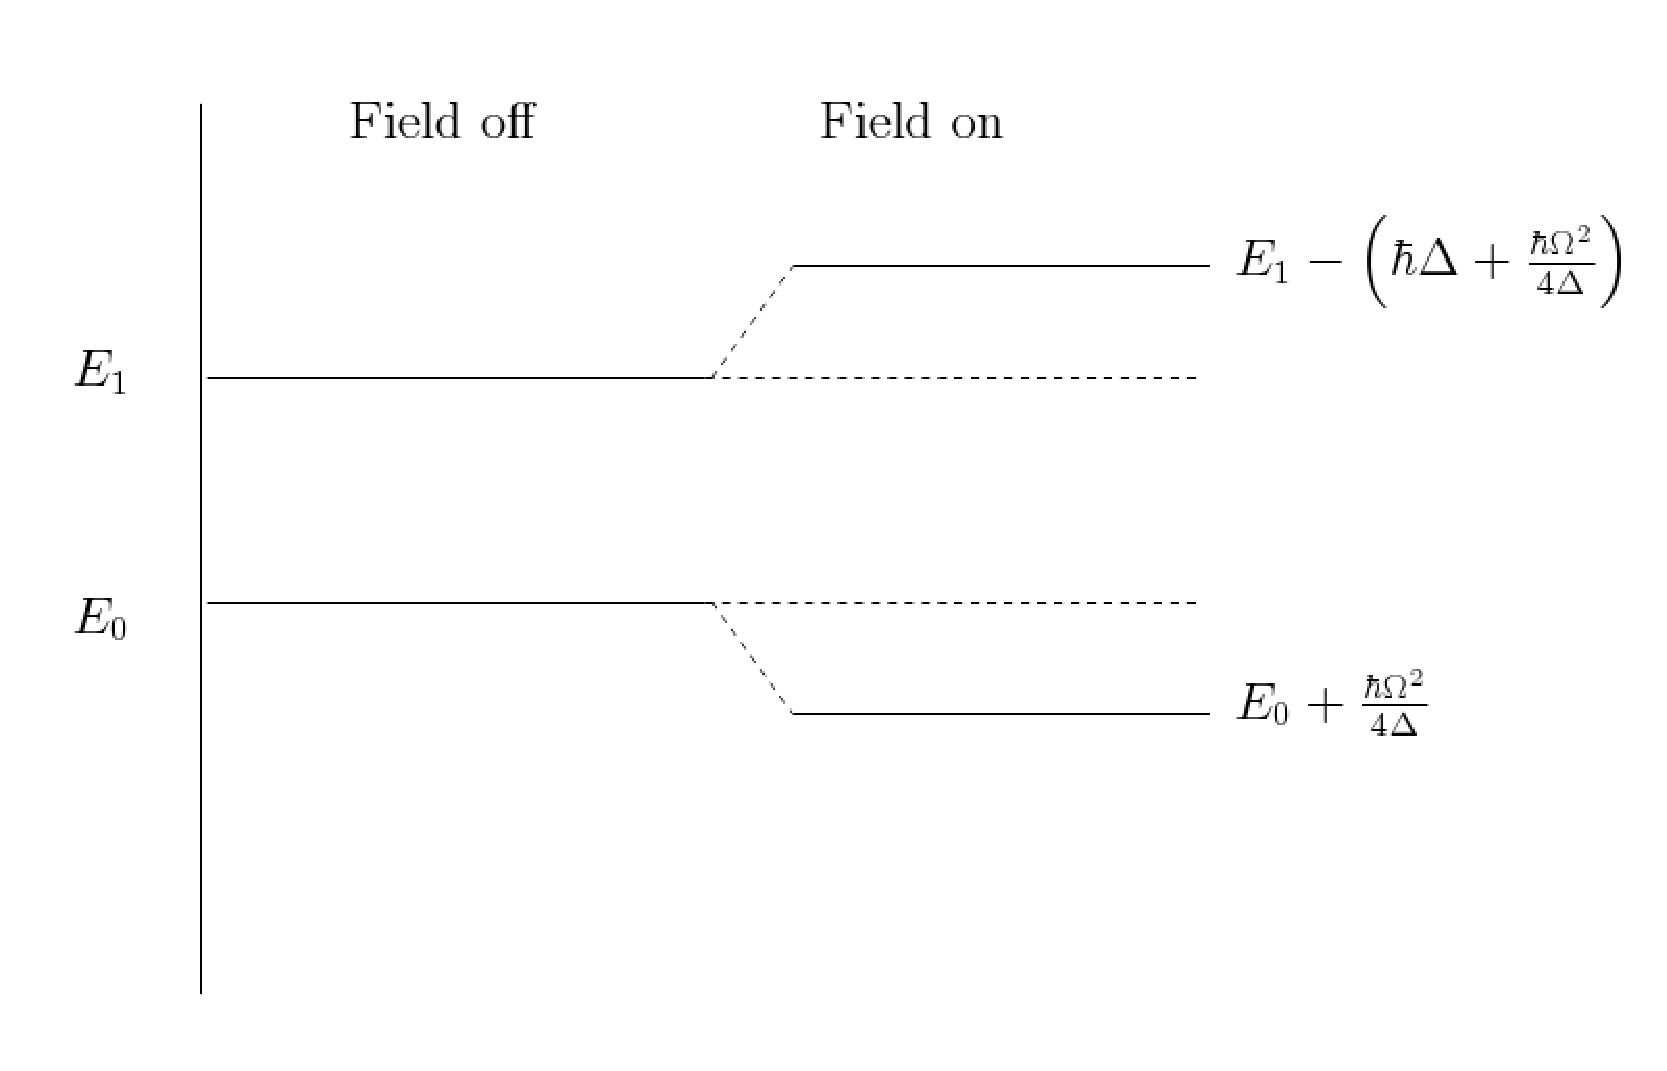
\psfig{file=jpegs/chapter-intro/fig1.eps,height=3.6in,width=5.3in}
\caption{Energies for the two-level problem with the laser field turned off and then on with negative detuning. The energy levels $E_0$ and $E_1$ are shifted due to the interaction between the system and the laser field.}
\label{fig:dressed:states:chapter-intro}
\end{figure}
Plugging these into Eqn~\ref{eq:2level:dynamics:chapter-intro} gives us (after dropping the primes)
\begin{eqnarray}
i\hbar \frac{d}{dt}\langle 0|\psi\rangle = \left( \frac{P^2}{2M} + E_0 \right) \langle 0|\psi\rangle + \frac{\hbar \Omega}{2} \langle 1|\psi\rangle S(t), \nonumber \\
i\hbar \frac{d}{dt}\langle 1|\psi\rangle = \left( \frac{P^2}{2M} + E_1 \right) \langle 1|\psi\rangle - \hbar \Delta \langle 1|\psi\rangle + \frac{\hbar\Omega}{2}\langle 0|\psi\rangle S^*(t), \nonumber \\
S(t)= e^{-i\Delta t} \left[ e^{i \left( kz-\omega t \right)}+  e^{-i \left( kz-\omega t \right)} \right] e^{-i\omega_0 t}.
\label{eq:2level:transformed:chapter-intro}
\end{eqnarray}
We now apply the R.W.A. to $S(t)$, and all the time dependent terms average out, leaving only the $z$-dependent terms, which can be treated as unity, giving us
\begin{eqnarray}
i\hbar \frac{d}{dt}\langle 0|\psi\rangle = \left( \frac{P^2}{2M} + E_0 \right) \langle 0|\psi\rangle + \frac{\hbar \Omega}{2} \langle 1|\psi\rangle, \nonumber \\
i\hbar \frac{d}{dt}\langle 1|\psi\rangle = \left( \frac{P^2}{2M} + E_1 \right) \langle 1|\psi\rangle - \hbar \Delta \langle 1|\psi\rangle + \frac{\hbar\Omega}{2}\langle 0|\psi\rangle.
\label{eq:2level:transformed:rwa:chapter-intro}
\end{eqnarray}
This is the Schr\"odinger dynamics of an effective time independent Hamiltonian $H_{eff}$ which is given by 
\begin{equation}
H_{eff} = \frac{P^2}{2M}+
\left( \begin{array}{cc}
E_0 & 0\\
0 & E_1
\end{array}
\right) + \frac{\hbar}{2} \left( \begin{array}{cc}
0 & \Omega \\
\Omega & -2 \Delta
\end{array}
\right).
\label{eq:3lvl:hamilt:chapter-intro}
\end{equation}
The energy eigenvalues are given by 
\begin{equation}
E'_{0,1}=\frac{P^2}{2M}+E_{0,1}+ \frac{\hbar}{2} \left( -\Delta \pm \sqrt{\Omega^2 + \Delta^2} \right).
\label{eq:diag:chapter-intro}
\end{equation}
The eigenvectors, $|\psi'_0 \rangle$ and $|\psi'_1 \rangle$, are referred to as 'dressed states'. The eigenvector corresponding to $E'_0$ is 
\begin{equation}
|\psi'_0 \rangle = \langle 0 | \psi \rangle \left( \begin{array}{c}
                                                 1 \\
						 W(\Omega/\Delta)
                                                \end{array}\right),
\end{equation}
where
\begin{equation}
W\left(\Omega/\Delta\right) \equiv \frac{-1+\sqrt{1+\left( \Omega/\Delta \right)^2}} {\Omega/\Delta}.
\label{eq:w:chapter-intro} 
\end{equation}
If the detuning $\Delta$ is large enough compared to $\Omega$, we can neglect $W$ 
\footnote{$\lim_{x \to 0}W(x)=0$ by l'H\^{o}pital's rule} and 'adiabatically eliminate' the excited state~\cite{graham}, yielding the eigenstate as just the ground state $\langle 0|\psi\rangle$. Thus, the excited state is eliminated and the system remains in the ground state with an effective Hamiltonian given by $E'_0$ in Eqn~\ref{eq:diag:chapter-intro} for the external degrees of freedom, ie
\begin{equation}
H_{eff}=E'_0=\frac{P^2}{2M}+E_0+ \frac{\hbar}{2} \left( -\Delta + \sqrt{\Omega^2 + \Delta^2} \right).
\label{eq:effham:chapter-intro}
\end{equation}
In the limit where $\Omega \ll |\Delta|$, we can simplify $E'_0$ by binomial approximation applied to Eqn~\ref{eq:effham:chapter-intro}.  This yields the 'Reduced Atom' Hamiltonian
\begin{equation}
H_{red}=\frac{P^2}{2M}+E_0+\frac{\hbar \Omega^2}{4\Delta},
\label{eq:redhamilt:chapter-intro}
\end{equation}
where
\begin{equation}
\delta E _0 = \frac{\hbar \Omega^2}{4\Delta},
\label{eq:starkshifts:chapter-intro}
\end{equation}
is the A.C stark shift~\cite{metcalf:vanderstraten}, and $E'_0=E_0 + \delta E_0$. 

From Eqn~\ref{eq:rabifreq:chapter-intro}, we see that the Rabi frequency $\Omega$ follows the same profile as the electric field. Therefore $\Omega^2$ follows the intensity profile of the laser in the space where the atom(s) are unconfined. A spatially inhomogeneous light field varying adiabatically in space, will thus produce a dressed state potential profile $V(x) =  \frac{ \hbar \Omega^2(x)}{4\Delta}$, the upper term of Eqn~\ref{eq:starkshifts:chapter-intro} (See Fig~\ref{fig:dressed:states:chapter-intro}). Here, the spatial variation of the electric field in $x$ produces spatial variations in $\Omega$. The resultant effective Hamiltonian, simplified from Eqn~\ref{eq:2lvl:hamilt:chapter-intro} to Eqn~\ref{eq:redhamilt:chapter-intro}, describes the translational motion of the atoms and is called the 'Reduced Atom' Hamiltonian
\begin{equation}
H_{red}(x) = \frac{P^2}{2M} + E_0 + V(x).
\end{equation}
The force resulting from the gradient is called the dipole force. If the beam intensity profile is tempered, and if $\Delta<0$, the dipole force is responsible for trapping the atoms around the maxima of the intensity profile of the laser in a particular direction. Double well potentials can be generated by bringing two laser beams with Gaussian intensity cross sections close together~\cite{dudarev:entanglement}. Standing waves produced by such lasers in counter propagating directions will produce spatially periodic optical lattice potentials~\cite{Deutsch:Jessen}~\cite{oplattice:bloch}. We will deal with both systems in this dissertation. Henceforth, all Hamiltonians in this dissertation will be presented in reduced atom form unless otherwise stated. 

To get an idea of the experimental parameters, we look at  $^{85}$Rb  atoms subjected to laser light. The electron configuration for Rubidium is $[Kr] 5s^1$. Thus, the angular momentum of the outermost electron $L=0$, and, with spin $S=1/2$ and spin-orbit coupling producing vector angular momenta ${\bf J}={\bf L}+{\bf S}$~\cite{rbdata}, we have $ J=1/2$ from the Clebsch-Gordan coefficients~\cite{sakurai}. Following the standard $^{2S+1}L_J$ convention used in atomic physics to denote $LS$ coupled orbitals, the lowest such orbital for  $^{85}$Rb is $5$ $^2S_{1/2}$. The next levels are $5$ $^2P_{1/2}$ and $5$ $^2P_{3/2}$. The transitions between these states are denoted by the $D_1$ ($5$ $^2S_{1/2}$ $\leftrightarrow$ $5$ $^2P_{1/2}$) and $D_2$ ($5$ $^2S_{1/2}$ $\leftrightarrow$ $5$ $^2P_{3/2} $) lines. 

Hyperfine structure is generated by the coupling between this angular momentum and the nuclear angular momentum ${\bf I}$, where $I=5/2$ for  $^{85}$Rb~\cite{rbdata}. We denote this total angular momentum by ${\bf F}={\bf J}+{\bf I}$. Using the Clebsch-Gordan coefficients, we get $ |J-I| \leq F \leq J+I$~\cite{sakurai}. Thus, for the $^{85}$Rb ground state, $5 ^2S_{1/2}$, we get the allowed values of $F=\left[ 2,3\right]$. For the $D_1$, excited state, $F=\left[2,3\right]$, and $F=\left[1,2,3,4 \right]$ for the $D_2$ excited state. The hyperfine splitting is calculated from the Hamiltonian given in~\cite{rbdata} and the $D_2$ levels shown in Fig~\ref{fig:rblevels}. We detune away from this resonance of $\simeq 1.6$ $eV$ which will require a red laser of about $780.241$ $nm$ (this line is more relevant than the $D_1$ line on account of its cycling transition being the one used for cooling and trapping the atom~\cite{rbdata}). The dipole matrix element is of the order of  $er_0$ where $r_0$ is the Bohr Radius~\cite{rbdata}. From Eqn~\ref{eq:rabifreq:chapter-intro}, we get $\hbar \Omega\simeq \alpha E_0$ where $\alpha\equiv e r_0 \simeq 10^{-28}$ $Cm$. Typical laser beams of power $\simeq 10 mW$~\cite{raizen} with $1/e^2$ area~\cite{encyclopedia:laser} of $\simeq 200\pi$ $(\mu m)^2$~\cite{raizen} gives us an energy flux $S\simeq 1.6 {\times} 10^{-2}$ $\frac{mW}{(\mu m)^2}$. Using the relation $S=\epsilon_0 c E^2_0$~\cite{jackson}, we get $E_0\simeq 10^5$ in SI units. Thus, $\hbar\Omega\simeq 5$ $\mu eV$, which is significantly smaller than typical detunings of $\hbar \Delta \simeq 0.1$ $meV$~\cite{steck}. Thus, reduced atom Hamiltonians are realized. Keeping the system at integer momentum $F=2$ means that the system is bosonic. Thus, a many-body system of such atoms will require boson statistics.

\begin{figure}
\hspace*{-0.1in}
\ 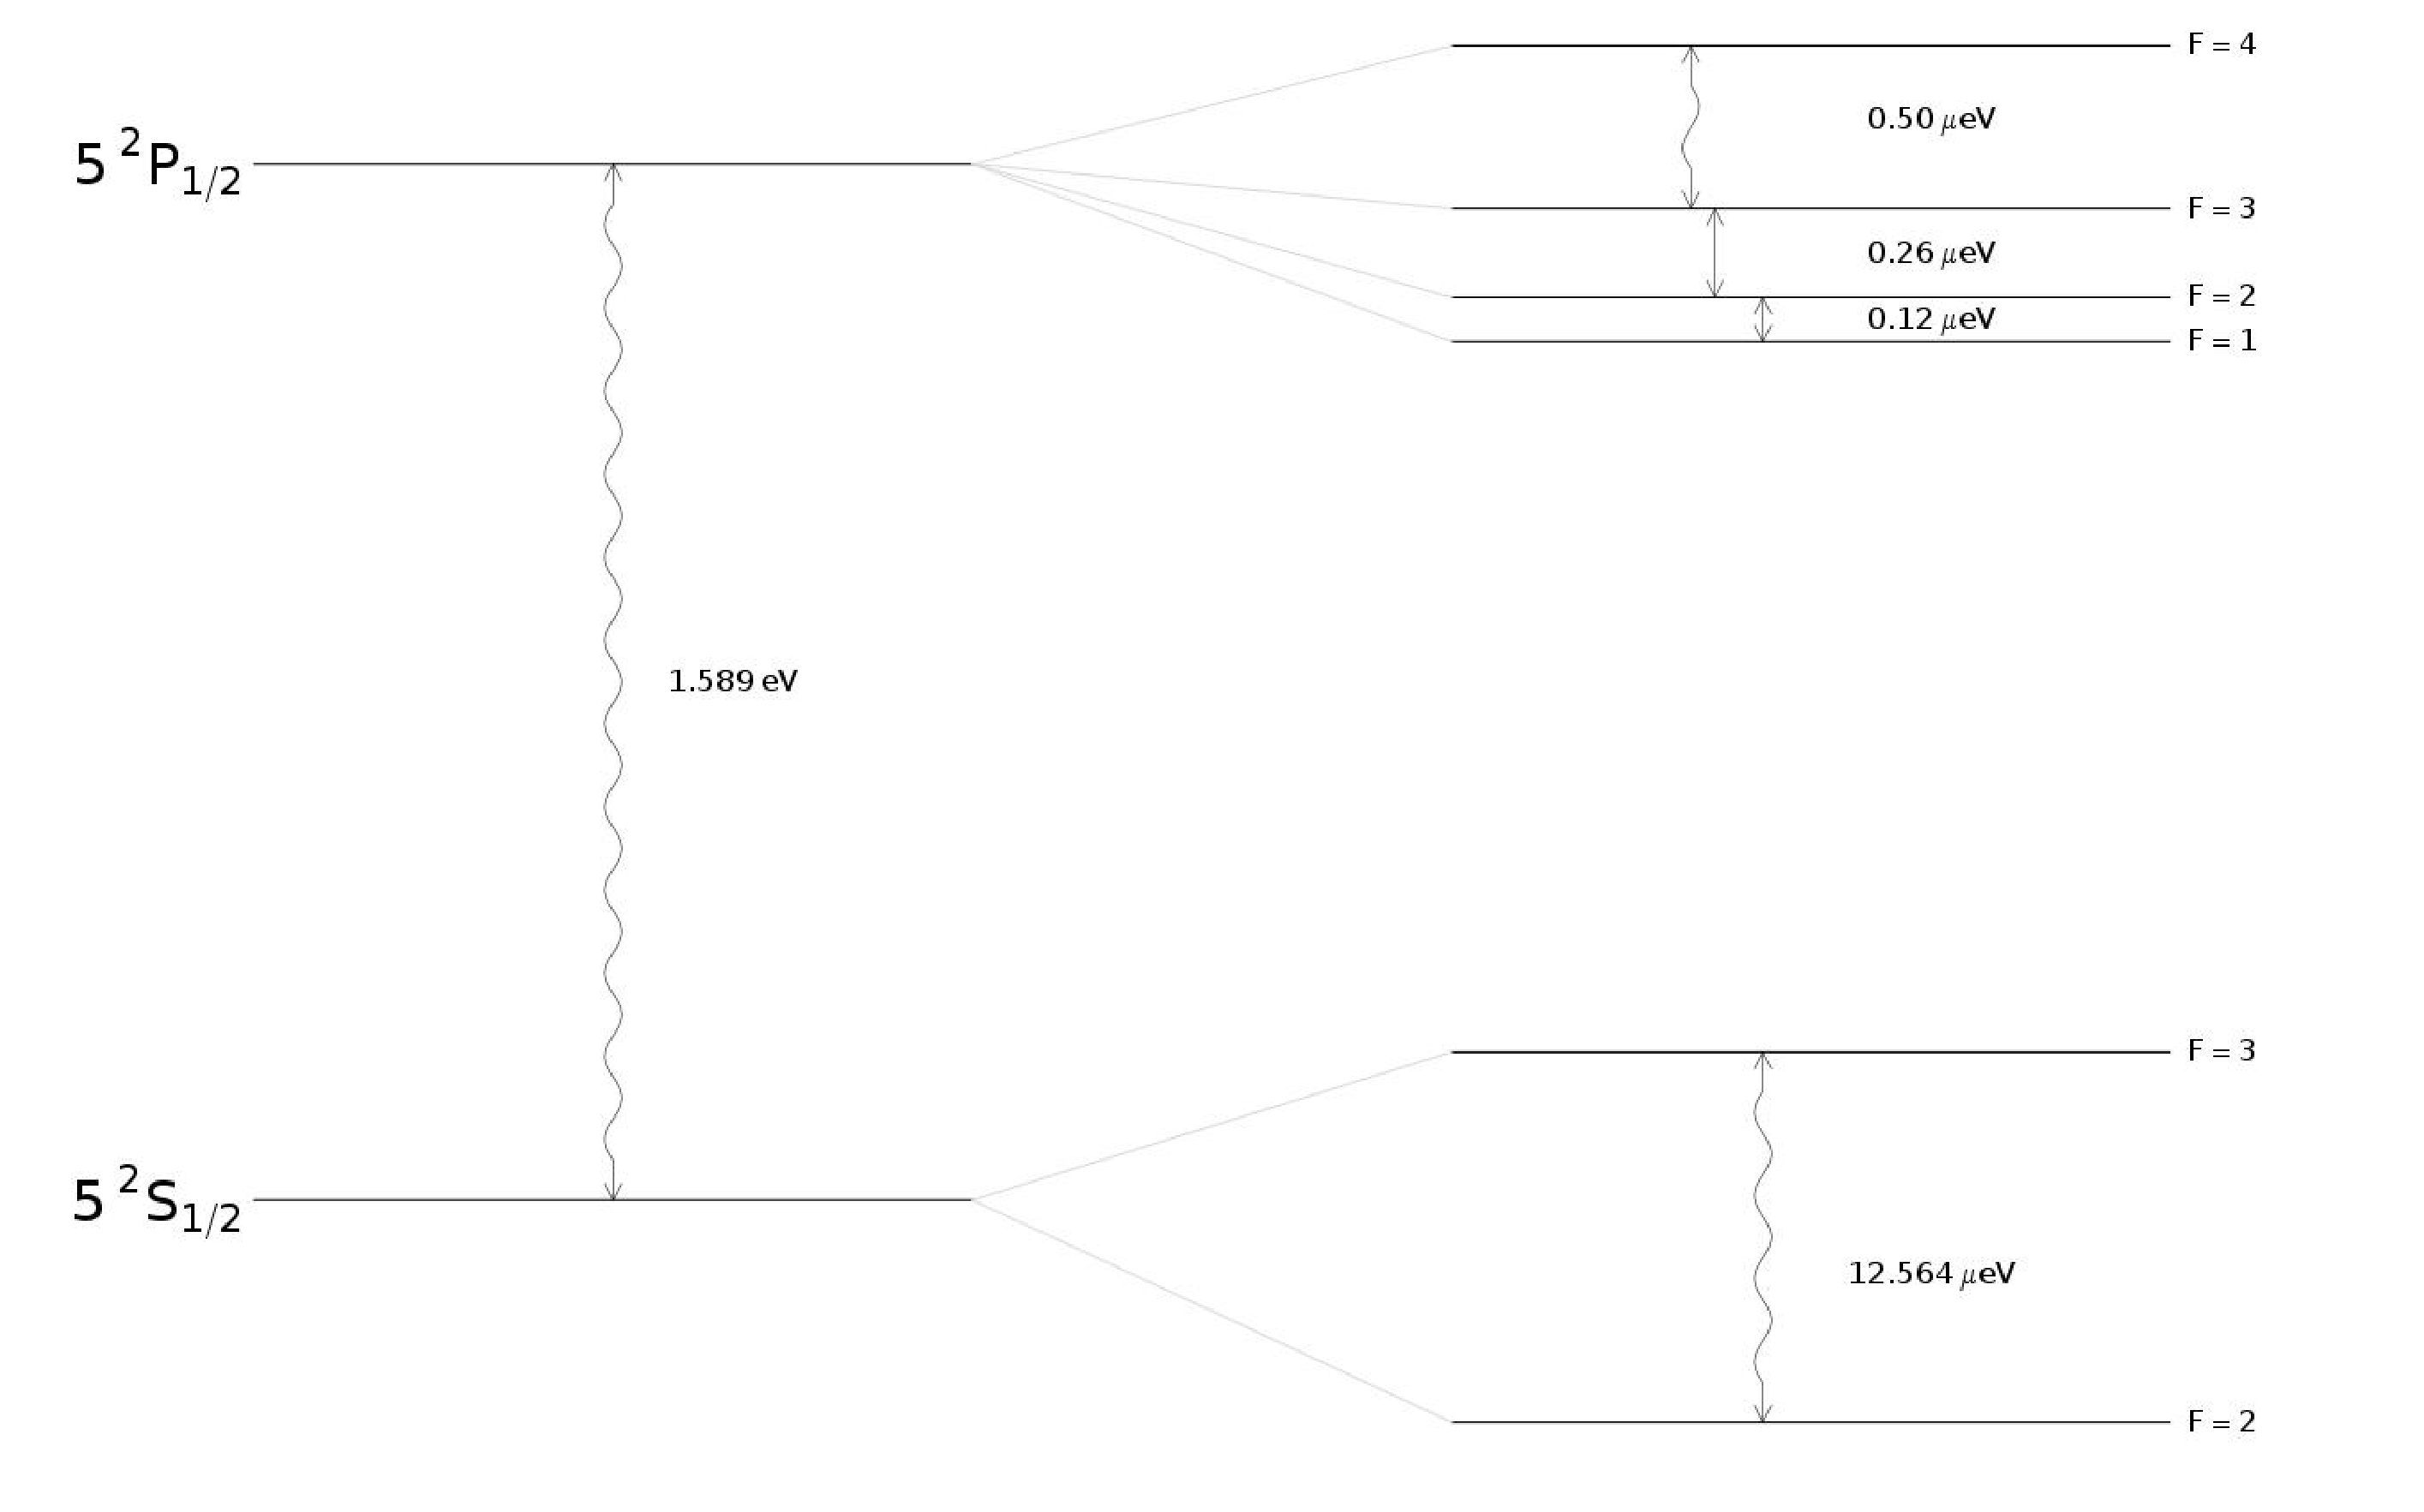
\psfig{file=jpegs/chapter-intro/fig_rblevels.eps,height=5.0in,width=5.9in}
\caption{Energy levels for the $D_2$ transition lines of  $^{85}$Rb }
\label{fig:rblevels}
\end{figure}

\subsection{Magnetic Confinement and Atom Chips}
\label{chapter-intro:section:atomchip:subsec:2lvl}
We can infer from the section above that a laser beam with a Gaussian cross section, once diffracted into two beams by diffraction methods, can be used to generate a double well system whose well separation is of the order of the wavelength of light used ($\simeq 1000$ $nm$). Sub-wavelength separations are not possible as diffraction effects will merge the double wells. For smaller length scales, we will have to exploit the dipole interactions with strong magnetic fields in atomic systems. Quadrupole magnetic fields can create zones where the magnitude of the field is a local minimum, thereby trapping the atoms, and a homogeneous RF oscillator producing a time dependent magnetic field breaks the rotational symmetry that produces the double well. These systems have been generated in the laboratory using atom chips for the purposes of matter interferometry~\cite{doublewell:chip}~\cite{doublewell:chip:nature}. Therefore, a discussion of these systems and the confinement produced by them is warranted.

Magnetic trapping of neutral atoms occurs due to the Zeeman effect, which cause the degeneracy in the hyperfine manifolds to split. For a $^{85}Rb$ atom, we have seen how the hyperfine levels $F$ are obtained from the spin-orbit-nuclear coupling (see section~\ref{chapter-intro:section:lightatom:subsec:2lvl} and~\cite{rbdata}). When an external magnetic field ${\bf B}$ is applied, the Hamiltonian describing the atomic interaction with the magnetic field is given by
\begin{eqnarray}
H=\frac{\mu_B}{\hbar} \left( g_S {\bf S}+g_L{\bf L}+g_I{\bf I}\right) \bullet {\bf B}, \nonumber \\
  = \frac{\mu_B}{\hbar} \left( g_S  S_z+g_L  L_z+g_I I_z\right)  B_z.
\end{eqnarray}
Here, the quantities $g_{(L,S,I)}$ are the Lande g-factors for the orbital, spin and nuclear angular momenta respectively, $\mu_B $ is the Bohr magneton, and the magnetic field is chosen to be in the $z-$direction. The g-factors $g_L\simeq1$, $g_s\simeq 2$, and $g_I\simeq -0.0003$~\cite{rbdata}. If the energy shift due to the magnetic field is small compared to the fine, and hyperfine splitting, then ${\bf F}={\bf L}+{\bf S}+{\bf I}$ is a 'good quantum number' and the Hamiltonian simplifies~\cite{rbdata} to
\begin{equation}
H = \mu_B g_F B_z,
\end{equation}
where
\begin{multline}
g_F \simeq \frac{F(F+1)-I(I+1)+J(J+1)}{2F(F+1)} \\
  \left\{1+ \frac{J(J+1)+S(S+1)-L(L+1)}{2J(J+1)}  \right\}.
\end{multline}
  As detailed in section~\ref{chapter-intro:section:lightatom:subsec:2lvl}, $F=2$, $L=0$, $I=5/2$, and $J=S=1/2$ for the $5$ $^2S_{1/2}$ state of $^{85}Rb$, thus $g_F\simeq-1/3$. For weak magnetic fields, $H$ perturbs the zero-field eigenstates of the hyperfine manifold. Thus, first order perturbation theory gives us~\cite{sakurai} energy shifts
\begin{equation}
\Delta E_{F,m_F} = \mu_B g_F m_F B_z ,
\label{eq:atomic:levels:chapter-intro}
\end{equation}
where $m_F$ are integers in the range $\left[-F, F \right]$. If the magnetic field is spatially varying, we now have the initial Hamiltonian for our system~\cite{lesanovsky:maghamilt}
\begin{equation}
H_{init}(t) = g_F \mu_B {\bf B}({\bf r},t) \bullet {\bf F}.
\label{maghamilt:chapter-intro}
\end{equation}
Equation~\ref{maghamilt:chapter-intro} represents the most general Hamiltonian of neutral atoms in magnetic fields. Now, the magnetic field is split into two terms,
\begin{equation}
{\bf B}({\bf r},t) =  {\bf B}_s({\bf r}) + {\bf B}_{rf}({\bf r},t).
\end{equation}
Here, ${\bf B}_s({\bf r})$ is a field that generates an Ioffe-Pritchard trap~\cite{pethick:bec}~\cite{Pritchard:trapgradients} with a global minimum in $|{\bf B}|$ at ${\bf r}=0$, and ${\bf B}_{rf}({\bf r},t)$ is a radio-frequency field that is linearly polarized in the $x-$direction. Thus,
\begin{eqnarray}
  {\bf B}_s({\bf r}) = Gx {\bf e}_x   -Gy {\bf e}_y   +B_I{\bf e}_z, \nonumber \\ 
 {\bf B}_{rf}({\bf r},t) = \frac{B_{rf}}{2}\left( e^{i\omega t}+ e^{-i\omega t} \right) {\bf e}_x,
 \label{eq:magfields:chapter-intro}
\end{eqnarray}
with $G$ being the gradient of the Ioffe field. The Hamiltonian in Eqn~\ref{maghamilt:chapter-intro} is now split up into two parts,
\begin{eqnarray}
H_{init}(t) = H_s + H_{rf}(t), \nonumber \\
H_s =  g_F \mu_B {\bf B}_s({\bf r}) \bullet {\bf F}, \nonumber \\
H_{rf}(t) = g_F \mu_B {\bf B}_{rf}({\bf r},t) \bullet {\bf F}.
\label{maghamilt:split:chapter-intro}
\end{eqnarray}
The Schr\"odinger equation for this system can be written as 
\begin{equation}
\left( H_s + H_{rf}(t) - i\hbar \frac{\partial}{\partial t} \right) |\psi(t)\rangle = 0.
\label{maghamiltdyn:split:chapter-intro}
\end{equation}
We transform each parts of Eqn~\ref{maghamiltdyn:split:chapter-intro} to a basis where $H_s$ is diagonal. If the transformation matrix is denoted by $U_s$, then
\begin{eqnarray}
U_s = \exp{\left( iF_z \phi \right)}\exp{\left( iF_y\beta\right)}, \nonumber \\
\cos{\beta} = \frac{B_I}{|{\bf B}_s({\bf r})|}, \nonumber \\
\sin{\beta} = - \frac{G\rho}{|{\bf B}_s({\bf r})|},
\label{eq:beta:chapter-intro}
\end{eqnarray}
where we have used cylindrical polar coordinates $\left[ x, y, z \right]=\left[ \rho \cos{\phi}, \rho \sin{\phi}, z \right]$. After applying the transformation, $H'_s=U^\dagger_s H_s U_s$ simplifies to 
\begin{equation}
H'_s = |{\bf B}_s({\bf r})|F_z,
\label{eq:hstrans:chapter-intro}
\end{equation}
and $H'_{rf}=U^\dagger_{rf} H U_s$. Thus, 
\begin{equation}
\left( H'_s + H'_{rf}(t) - i\hbar \frac{\partial}{\partial t} \right) |\psi(t)\rangle = 0.
\label{maghamiltdyntrans:split:chapter-intro}
\end{equation}
We proceed from here by first simplifying $H'_s$. We do so by applying a second transformation $U_r$ that rotates the system to the phase of the radio-frequency field. Thus, $U_r = \exp{\left(-i\frac{g_F}{|g_F|} F_z \omega t \right)}$, and the transformed Hamiltonian $H''_s$ is given by
\begin{equation}
H''_s - i\hbar \left( \frac{\partial}{\partial t} \right)'' =U^\dagger_r H'_s U_r - i\hbar U^\dagger_r \frac{\partial}{\partial t} U_r.
\end{equation}
Upon applying this transformation, we get
\begin{equation}
H''_s - i\hbar \left( \frac{\partial}{\partial t} \right)'' = \left( g_F  \mu_B |{\bf B}_s({\bf r})| -\frac{g_F}{|g_F|} \hbar \omega   \right).
\label{eq:hstransfinal:chapter-intro}
\end{equation}
Now, we apply all of the above transformations to $H_{rf}$. Thus, we get $H''_{rf}(t) = U^\dagger_r H'_{rf}(t)U_r$, where
\begin{multline}
H''_{rf}(t) =   \frac{g_F \mu_B B_{rf}}{2}\left( e^{i\omega t}+ e^{-i\omega t} \right) \times   \\
\exp{\left(i\frac{g_F}{|g_F|} F_z \omega t \right)} \exp{\left(- iF_y\beta\right)}  \exp{\left(- iF_z \phi \right)} \times \\
   F_x   \exp{\left( iF_z \phi \right)}\exp{\left( iF_y\beta\right)}  \exp{\left(-i\frac{g_F}{|g_F|} F_z \omega t \right)}.
\end{multline}
This equation can be evaluated by applying the Baker-Campbell-Hausdorff formula on each pair of exponentials on either side of $F_x$~\cite{sakurai}, and simplifying the expansion using the angular momentum commutation relations $\left[ F_i, F_j \right] = i\hbar \epsilon_{ijk} F_k$ (where the square bracket indicates $\left[ F_i, F_j \right] \equiv F_iF_j-F_jF_i$, and $\epsilon_{ijk}$ is the Levi-Civita symbol). After applying the rotated wave approximation (RWA) and neglecting terms that oscillate with frequency of $2\omega$ or higher (cf section~\ref{chapter-intro:section:lightatom:subsec:2lvl}), we get 
\begin{eqnarray}
H''_{rf}(t) = \frac{g_F \mu_B}{2} \bar{{\bf B}} \bullet {\bf F}, \nonumber \\
\bar{{\bf B}} = B_{rf} \left( \cos{\beta} {\bf e}_x + \sin{\phi}\sin{\beta}{\bf e}_y \right).
\label{eq:hrftransfinal:chapter-intro}
\end{eqnarray}
We now obtain an expression for the rotated wave Hamiltonian $H''$ for the whole system by applying Eqns~\ref{eq:hstransfinal:chapter-intro} and~\ref{eq:hrftransfinal:chapter-intro} to Eqn~\ref{maghamiltdyn:split:chapter-intro}. After dropping the primes, this gives us (for the LHS of Eqn~\ref{maghamiltdyn:split:chapter-intro})
\begin{equation}
H= \left( g_F  \mu_B |{\bf B}_s({\bf r})| -\frac{g_F}{|g_F|} \hbar \omega   \right) + \frac{g_F \mu_B}{2} \left(\bar{B}_x F_x + \bar{B}_y F_y  \right).
\label{maghamilt:rwa:chapter-intro}
\end{equation}
Thus, the solution to the dynamics of Eqn~\ref{maghamiltdyn:split:chapter-intro} can be reduced to diagonalizing the time independent rotated wave Hamiltonian $H$. This can be done in the $m_F$ representation by writing out the matrix elements using the ladder     
operator relations for the angular momentum ${\bf F}$~\cite{sakurai}. We now diagonalize this Hamiltonian in a two level system similar to the one in section~\ref{chapter-intro:section:lightatom:subsec:2lvl}, where we select two consecutive $m_F$ states. The adiabatic potential thus obtained is~\cite{lesanovsky:maghamilt}
\begin{equation}
V({\bf r}) = g_F m_F \mu_B \sqrt{\left( |{\bf B}_s({\bf r})|-\frac{\hbar \omega}{|g_F \mu_B|} \right)^2+ \frac{1}{4} \left( \bar{B}_x^2 + \bar{B}_y^2 \right)}.
\end{equation}
This can be simplified in cylindrical polar coordinates $\left[\rho, \phi \right]$ by using the definitions in Eqns~\ref{eq:beta:chapter-intro} and~\ref{eq:hrftransfinal:chapter-intro} to yield
\begin{equation}
V({\bf r}) = g_F m_F \mu_B \sqrt{\left[ |{\bf B}_s({\bf r})|-\frac{\hbar \omega}{|g_F \mu_B|} \right]^2 + \left[\frac{B_{rf}}{2|{\bf B}_s({\bf r})|} \right]^2 \left( B^2_I +G^2 \rho^2 \sin^2\theta \right)}.
\end{equation}
The minima of this potential can be found at $\theta = \left[0, \pi \right]$ (provided that $g_F m_F >0$). If the radius $\rho \ll B_I/G$, we can approximate
\begin{eqnarray}
V(\rho) \simeq g_F m_F \mu_B \sqrt{\frac{G^4}{B^2_I}\left(\frac{\rho^2-\rho^2_0}{2} \right)^2+B^2_0}, \nonumber \\
\rho^2_0 \equiv \frac{B^2_{rf}-B^2_c}{2G}, \nonumber \\
B_0 \equiv \frac{B_{rf}}{4B_I}\sqrt{4B^2_I + B^2_C -2 G^2\rho^2_0}, \nonumber \\
B_c \equiv 2\sqrt{B_I \left( \frac{g_F\mu_B B_I -\hbar\omega}{|g_F\mu_B|}\right)}.
\label{eq:magpot:chapter-intro}
\end{eqnarray}
From Eqns~\ref{eq:magpot:chapter-intro}, we can clearly see that the potential $V(\rho)$ is a one-dimensional double well potential along the polar direction of the 
the potential minima. The well minima can be found at $\rho=\pm \rho_0$ about the origin. Transforming to the $\theta= 0$ or $\pi$ axis, we get 
\begin{equation}
V(x) = g_F m_F \mu_B \sqrt{\frac{G^4}{B^2_I}\left(\frac{x^2-x^2_0}{2} \right)^2+B^2_0}.
\label{eq:1dmagpot:chapter-intro}
\end{equation}
where $x_0=\rho_0$. For a sufficiently high Ioffe field $B_I$ , $\left(G^2x^2_0/2B_I\right) \ll B_0$~\cite{pethick:bec}~\cite{doublewell:chip}, and Eqn~\ref{eq:1dmagpot:chapter-intro} can be expanded binomially to get an equation of the type
\begin{equation}
 V(x)= V_0 (-2{\bar x}^2 + {\bar x}^4),
\end{equation}
where we have dropped overall constant terms, and defined
\begin{eqnarray}
 V_0 \equiv \frac{g_F m_F \mu_B G^4 x^4_0}{8B_0B^2_I}, \nonumber \\
 {\bar x}\equiv \frac{x}{x_0}. 
 \label{eq:welldepth:chapter-intro}
 \end{eqnarray}
Note that ${\bar x}$ is dimensionless, and $V_0$, which gives us the well-depth, has the dimensions of energy. Thus, after adding the translational degrees of freedom ($\frac{p^2}{2m}$) to the above simplification of the atomic interaction with the magnetic field, we can get a 'reduced atom' Hamiltonian of a particle in a quartic double well whose minima can be found at $\pm x_0$. 

Such potentials have been achieved with atom chip systems by Schumm et al in 2006~\cite{doublewell:chip}~\cite{doublewell:chip:nature}. In these experiments, an atom chip containing lithographically etched DC current-carrying micro-wires (which, when combined with an external pair of Helmholtz coils, generates the quadrupole field for an Ioffe-Pritchard trap~\cite{pethick:bec}) together with a micro-wire carrying an ac current (for the RF field), confines a BEC in a double well potential immediately below the chip. The radio frequencies of about $500$ $KHz$ and magnetic fields $B_{rf}\equiv 1$ Gauss in a standard Ioffe-Pritchard trap. We note that, from Eqn.~\ref{eq:magpot:chapter-intro}, $x_0=\sqrt{\left(B_{rf}^2-B^2_c\right)/2G}$. The parameters in the double well atom chip of Schumm et al produce an $x_0$ of the order of $10$ $\mu m$. If we desire a well-separation of $L_u=50$ $nm$, and a potential well depth ($V_{max}(x)$ of Eqn~\ref{eq:1dmagpot:chapter-intro}) that is of the order of $E_u=\frac{\hbar^2}{2mL_u^2}$ for the mass $m$ of a $^{85}Rb$ atom, then we need to solve the simultaneous equations
\begin{eqnarray}
V_0=E_u \nonumber \\
x_0=L_u.
\label{eq:magpot:roots:chapter-intro}
\end{eqnarray}
Using Eqns~\ref{eq:welldepth:chapter-intro} and~\ref{eq:magpot:chapter-intro}, we get
\begin{eqnarray}
\frac{g_Fm_F\mu_BG^4x^4_0}{8B_0B^2_I}=E_u=\frac{\hbar^2}{2mL^2_u} \nonumber \\
\frac{B^2_{rf}-B^2_c}{2G} = L^2_u,
\label{eq:magtrap:roots:chapter-intro}
\end{eqnarray}
where $B_0$ and $B_c$ are obtained from Eqns~\ref{eq:magpot:chapter-intro}. Equation~\ref{eq:magtrap:roots:chapter-intro} need to be solved for a given $L_u$, which we desire to be around $50$ $nm$, and for experimentally feasible parameters for the Ioffe-Pritchard trap. We choose to solve for the radial trap gradient $G$ and RF frequency $\omega$, with Ioffe Field $B_I=100$ $Gauss$ and RF field amplitude $B_{rf}=1$ $Gauss$ (both values are typical for this system~\cite{Pritchard:trapgradients}~\cite{doublewell:chip}). Figure~\ref{fig:magplots:chapter-intro} shows the progression towards the solution with graphs, where $V_0/E_u$ and $x_0/L_u$ are plotted as functions of $\omega$ for several values of $G$, ranging from $1$ $T/m$ to $10,000$ $T/m$ or $100$ $T/cm$. The intersection of the two graphs approaches unity in the latter most case, the exact solution for $G$ being $11303.375$ $T/m$ at $\omega=292.955314305$ $MHz$ (see Fig~\ref{fig:magplots:chapter-intro}.d). Radial field gradients much higher than this magnitude ($10^5$ $T/m$) have been reported for micro-magnets generated by wires lithographically etched on chips~\cite{drndic:higrad}~\cite{lev:highgrad}. Thus, one can readily obtain a stable double well system for the $F=2$, $m_F=-2$ state of $^{85}Rb$ within the required parameters. 
\begin{figure}
\ \psfig{file=jpegs/chapter-intro/fig_magplots.eps,height=5.2in,width=5.5in}
\caption{Graphical representation of the numerical solution to Eqn~\ref{eq:magpot:roots:chapter-intro} or~\ref{eq:magtrap:roots:chapter-intro}. Figures (a) through (d) plot dimensionless functions $V_0/E_u$ and $x_0/L_u$ as functions of the RF frequency $\omega$ for radial gradients $G=1$, $10$, $1000$ and $10^4$ $T/m$ respectively. The Ioffe Field $B_I=100$ $Gauss$ and RF field amplitude $B_{rf}=1$ $Gauss$. Both curves must intersect at unity for a solution, and Fig (d) shows plots for  the closest value of $G$ for which this happens (unity is indicated by a horizontal line). Fine-tuning the bisection method gives us the more accurate solution of $G=11303.375$ $T/m$ for $\omega=292.955314305$ $MHz$.}
\label{fig:magplots:chapter-intro}
\end{figure}
\section{Avoided Crossings and the Landau Zener Formula}
\label{chapter-intro:section:avcross}
An introduction to the concept of avoided crossings is provided here. We consider a quantum system described by a finite-dimensional Hilbert space $\cal H$. The Hamiltonian $H(\lambda)$ is parametrized by $\lambda$. The  'No-Crossing theorem' by von-Neumann and Wigner establishes that the variation of a single parameter in a finite-dimensional, 'general' Hermitian matrix ( a matrix with no relations between the matrix elements other than Hermiticity) cannot produce degeneracies in the eigenvalue spectrum. Thus, if symmetries (such as parity) exist, then eigenvalues may cross each other freely as the parameter is varied~\cite{vonneumann:wigner}. The symmetries cause eigenvalues to 'cross' each other in the parameter space, and breaking the symmetry causes those crossings to 'avoid' each other (see Fig~\ref{fig:2lvl:avcross:chapter-intro}), producing an 'avoided crossing' at that point. For a simple two level system similar to the one discussed in the last section, we have
\begin{equation}
H_0(\lambda)= \lambda \left( |0\rangle \langle 0| - |1\rangle \langle 1| \right),
\label{eq:hamilt:avcross:chapter-intro}
\end{equation}
where we have scaled our zero level for the energy to be midway between the unperturbed energies of the Hamiltonian. We apply a 'perturbation' $H'$ to this Hamiltonian, with the system now described by 
\begin{eqnarray}
H=H_0(\lambda)+H'(\delta), \nonumber \\
H'(\delta) = \delta \left( |0\rangle \langle 1| + |1\rangle \langle 0| \right),
\end{eqnarray}
or
\begin{equation}
H = \left( \begin{array}{cc}
            \lambda & \delta\\
	    \delta & -\lambda
           \end{array}\right).
\label{eq:fullhamilt:avcross:chapter-intro}
\end{equation}
\begin{figure}
\ 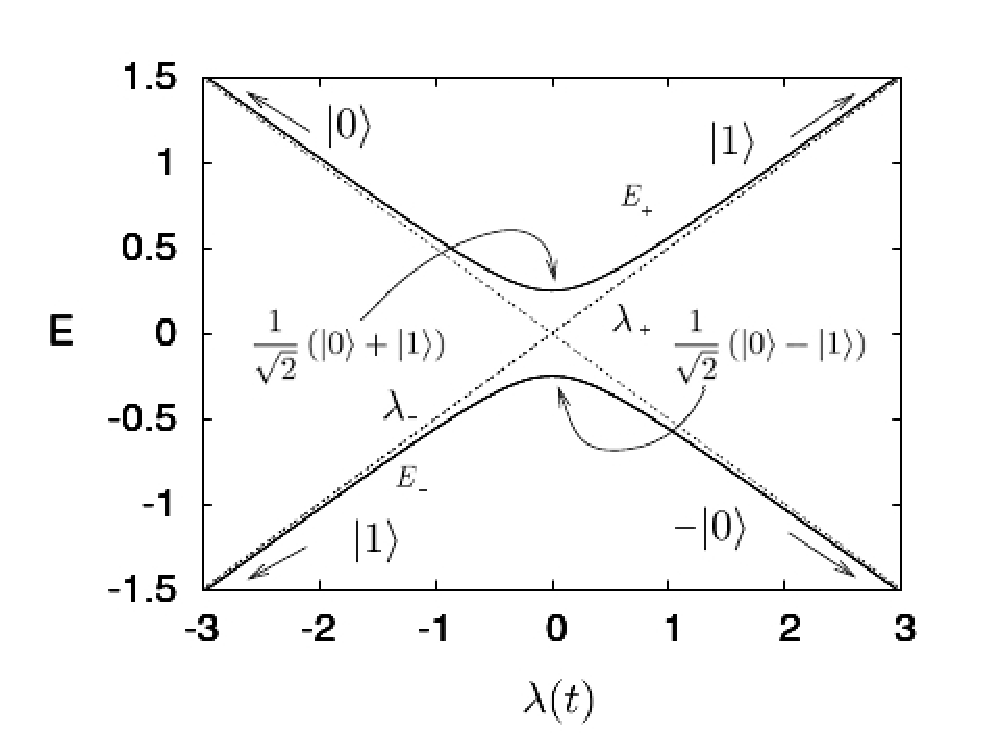
\psfig{file=jpegs/chapter-intro/fig_avcross.eps,height=3.0in,width=4.0in}
\caption{Adiabatic and diabatic eigenvalue curves of the 2 level quantum system. The diabatic ($\delta=0$) eigenvalues, $\lambda\pm$, are shown as dashed lines, and the adiabatic curves, $E_\pm$ are shown as solid curves (for $\delta=0.5$). Arrows indicate eigenstate character in the diabatic $\left[|0\rangle, |1\rangle \right]$ representation.}
\label{fig:2lvl:avcross:chapter-intro}
\end{figure}
The energy eigenvalues of this system are
\begin{equation}
E_\pm = \pm \sqrt{\lambda^2 + \delta^2},
\label{eq:2lvlen:chapter-intro}
\end{equation}
and are plotted in Fig~\ref{fig:2lvl:avcross:chapter-intro}. as a function of $\lambda$. They approach each other and 'avoid' a crossing at $\lambda=0$ by a factor of $2\delta$. We diagonalize the general Hamiltonian using the diagonal basis for $\lambda=0$. Thus, denoting the eigenstates as $| \lambda_\pm \rangle$, we have
\begin{equation}
| \lambda_\pm \rangle = C^0_\pm | (\lambda=0)_- \rangle + C^1_\pm | (\lambda=0)_+ \rangle,
\end{equation}
where 
\begin{equation}
| (\lambda=0)_\pm \rangle = \frac{1}{\sqrt{2}} \left( |0\rangle \pm |1\rangle \right).
\label{eq:avcross2lvl:chapter-intro}
\end{equation}
This Hamiltonian is transformed to the $|(\lambda=0)_\pm \rangle$ basis by $H^t(\lambda) = S^\dagger H(\lambda) S$, where
\begin{equation}
 S = \left(\begin{array}{cc}
        1 &1 \\
	-1 & 1
       \end{array}\right),
\end{equation}
yielding 
\begin{equation}
 H^t(\lambda)=\left(\begin{array}{cc}
                     \delta & -\lambda \\
		     -\lambda & -\delta
                    \end{array}\right),
\end{equation}
with the same eigenvalues. Solving for the $|\lambda_\pm \rangle$ eigenvectors, we get 
\begin{equation}
\frac{ C^0_\pm}{ C^1_\pm} = \frac{\lambda}{\delta \mp \sqrt{\lambda^2 + \delta^2}}.
\end{equation}
Now, we note the following limits for the ratio of the components of the eigenvector(s) viz.
\begin{equation}
\lim_{\lambda \to -\infty}\frac{ C^0_\pm}{ C^1_\pm} = \pm 1,
\label{eq:limits1:chapter-intro} 
\end{equation}
and
\begin{equation}
\lim_{\lambda \to +\infty}\frac{ C^0_\pm}{ C^1_\pm} = \mp 1 .
\label{eq:limits2:chapter-intro} 
\end{equation}
Thus, we see from Eqns~\ref{eq:limits1:chapter-intro} and ~\ref{eq:limits2:chapter-intro} that a state populated at $|0\rangle$ at $\lambda=-\infty$ will change character and switch over to $|1\rangle$ as the system adiabatically crosses $\lambda=0$ and approaches $\lambda=\infty$ and vice versa. Similarly, a state populated at $|1\rangle$ at $\lambda=-\infty$ will change character and switch over to $-|0\rangle$ as the system adiabatically crosses $\lambda=0$ and approaches $\lambda=\infty$ and vice versa. At $\lambda=0$, the states are given by Eqn~\ref{eq:avcross2lvl:chapter-intro}, and are thus 'mixed' between the two canonical basis states. 

This phenomenon is called an 'avoided crossing' and will be pivotal to our understanding of the full many-level dynamics of quantum control. The dynamics of a quantum controlled STIRAP will be described by a parameter $t_{fix}$ which will vary adiabatically, analogous to $\lambda$ in this section. The loss of symmetry will produce avoided crossings for particular values of $t_{fix}$ in the same region that the corresponding system loses the same symmetry (ie it is not integrable). The absence of invariant tori in the $\left[J, \Theta \right]$ space, a consequence of classical non integrability, causes the dynamics to transition to chaos in these regimes~\cite{reichl}. Thus, the presence of these avoided crossings and their effect on the spectral statistics on the system is a quantum manifestation of classical chaos, and their study merits interest in that context.

So far, we have ignored any temporal dependence in the variation of $\lambda$. We have implicitly relied on the fact that the quantum adiabatic theorem, first obtained by Max Born and Vladamir Fock in 1928, guarantees that a physical system remains in its instantaneous eigenstate if a given perturbation is acting on it slowly enough and if there is a gap between the eigenvalue and the rest of the Hamiltonian's spectrum~\cite{Born1928:adiabaticthm}. However, a distinction must be made between an \textit{adiabatic process}, where gradually changing conditions allow the system to adapt its configuration, hence modifying the probability density, and a \textit{diabatic process},  where rapidly changing conditions prevent the system from adapting its configuration during the process~\cite{kato:adiabaticthm}. In an adiabatic process, if the system starts in an eigenstate of the Hamiltonian, it will end in the corresponding eigenstate of the final Hamiltonian after a long time, changing character through any avoided crossings on the way in order to remain in it's adiabatic eigenvalue curve (in this case, $E_\pm$). However, this mechanism is disturbed if the parameters do not vary adiabatically. In such a case, the actual state of the system projects into other eigenstates of the Hamiltonian, causing the system to lose coherence~\footnote{In the extreme case of a diabatic process,  it's the probability density that remains unchanged. The system ends in a linear combination of states that sum to reproduce the initial probability density}. Thus, there is no eigenstate of the final Hamiltonian with the same functional form as the initial state~\cite{kato:adiabaticthm}. 

The criterion for a system to evolve adiabatically depends on several factors, such as the time scale $\tau$ for the variation of $\lambda$, as well as the energy gap between the eigenstate and the rest of the spectrum. For a two-level quantum system such as this, the Landau-Zener formula is an analytical solution that gives the probability of a diabatic transition between the two energy states. It was published separately by Lev Landau~\cite{landau:lzformula} and Clarence Zener~\cite{zener:lzformula} in 1932. Among the numerous derivations that have been published since then, we present a short summary of an elegant derivation of this relation by Wittig~\cite{wittig:lzformula}. If we plug in a time dependence on $\lambda$, and assume that the system starts at $t=-\infty$ in the lower energy eigenstate $|\lambda_-\rangle$, we can calculate the probability of finding the system in the upper energy eigenstate $|\lambda_+\rangle$ at $t=\infty$.  In order that the equations of motion for the system might be solved analytically, a set of simplifications are made, known collectively as the Landau-Zener approximation. The simplifications are as follows:
\begin{itemize}
 \item 
 The perturbation parameter in the Hamiltonian is a known, linear function of time, making this treatment semiclassical.
 \item
 The energy separation of the diabatic states varies linearly with time ie $\lambda(t)=\frac{\Gamma}{2} t$, where $2 \lambda$ is the energy level difference from Eqn.~\ref{eq:hamilt:avcross:chapter-intro}. Thus, $\Gamma$ is the rate at which the diabatic energy levels $\pm \lambda$ approach each other at the avoided crossing at $t=0$.
 \item
 The coupling in the diabatic Hamiltonian matrix is independent of time, ie $\delta$ is constant.
\end{itemize}

We now integrate the system in the canonical diabatic basis ($|0\rangle$, $|1\rangle$, which are the eigenstates for the diabatic case of $\delta=0$) by writing the state vector as
\begin{equation}
|\psi(t)\rangle = A(t) |0\rangle e^{-i\int^t dt' \lambda(t')} + B(t) |1\rangle e^{i\int^t dt' \lambda(t')}.
\end{equation}
Here, $\hbar=1$. Applying the Schr\"odinger equation $H|\psi(t)\rangle=i\frac{d}{dt}|\psi(t)\rangle$ for the Hamiltonian in Eqn.~\ref{eq:fullhamilt:avcross:chapter-intro}, and resolving the components in the diabatic basis, we get (in the interaction picture)
\begin{eqnarray}
\dot{A} = -i \delta B e^{2i\int^t dt' \lambda(t')}, \nonumber \\
\dot{B} = -i \delta A e^{-2i\int^t dt' \lambda(t')}.
\end{eqnarray}
Differentiating the above with respect to time and simplifying leads to
\begin{eqnarray}
\ddot{A} -2i\lambda(t) \dot{A} + \delta^2 A=0, \nonumber \\
\ddot{B} +2i\lambda(t) \dot{B} + \delta^2 B=0.
\end{eqnarray}
We now apply the itemized assumptions above and write out the equation for $B(t)$, getting
\begin{equation}
\ddot{B} + i\Gamma t \dot{B} + \delta^2 B=0.
\label{eq:eqn4B:chapter-intro}
\end{equation}
Here, $B(t)$ is the amplitude of the wavefunction in the 'excited state' $|1\rangle$. We desire to obtain an expression for $B(\infty)$, which will give us the probability of the system being measured at the excited state long after the avoided crossing at $t=0$ has been encountered. Assuming that $B(t)$ is nonvanishing for all finite times~\cite{wittig:lzformula}, we divide Eqn~\ref{eq:eqn4B:chapter-intro} by $dt/(Bt)$ and integrate over all times to get
\begin{equation}
i\Gamma \int^{B(\infty)}_1 \frac{dB}{B} = - \delta^2 \int^\infty_{-\infty} \frac{dt}{t} - \int^\infty_{-\infty} \left( \frac{dt}{t} \frac{\ddot{B}(t)}{B(t)}\right).
\label{eq:toint:chapter-intro}
\end{equation}
The limits of integration for $B$ are decided by the state populating the lower eigencurve of Fig~\ref{fig:2lvl:avcross:chapter-intro}. at $t=-\infty$, which has the characteristic of $|1\rangle$, making $B(-\infty)=1$. The first term in the RHS of Eqn~\ref{eq:toint:chapter-intro} can be integrated by the calculus of residues~\cite{arfken}. Thus,
\begin{eqnarray}
\int^\infty_{-\infty} \frac{dt}{t} = \lim_{\epsilon \to 0} \left( \int^\epsilon_{-\infty} + \int_\epsilon^\infty \right) \frac{dt}{t}, \nonumber \\
  = \left(\oint_C - \oint_{C_1}\right) \frac{dt}{t}.
\label{eq:int1:chapter-intro}
\end{eqnarray}
Here, the contours $C$ and $C_1$ are shown in Fig~\ref{fig:contours:chapter-intro}, and the sense of the integration indicated by arrows. The limit $\epsilon \rightarrow 0$ is implicit in the second equation. In the limit $R \rightarrow \infty$, Jordan's Lemma causes the $C$- contour integral to vanish~\cite{arfken}. In the contour $C_1$, $t=\epsilon e^{i\theta}$ with constant $\epsilon$. Thus, substitution into the contour integral gives $i\pi$, and Eqn~\ref{eq:toint:chapter-intro} simplifies to
\begin{equation}
\ln B(\infty) = - \pi \delta \tau - i \frac{\tau}{\delta}\int^\infty_{-\infty} \left( \frac{dt}{t} \frac{\ddot{B}(t)}{B(t)}\right),
\label{eq:eqn4lnB:chapter-intro}
\end{equation}
where $\tau=-\delta/\Gamma$. 

We now analytically continue the function $\frac{\ddot{B}(t)}{B(t)}$ into the complex plane~\cite{wittig:lzformula} and evaluate the integral. Evaluating the integral above  using the calculus of residues along the same contours as shown in Fig~\ref{fig:contours:chapter-intro} gives us
\begin{equation}
 \int^\infty_{-\infty} \left( \frac{dt}{t} \frac{\ddot{B}(t)}{B(t)}\right) =i \lim_{\epsilon \to 0} \int^0_\pi d\theta \frac{\ddot{B}(\epsilon)}{B(\epsilon)} + \lim_{R \to \infty} \int^\pi_0 i d\Theta \frac{\ddot{B}(R)}{B(R)}.
 \end{equation}
Note that the expression $\frac{\ddot{B}(t)}{B(t)}$ has no phase dependencies~\cite{wittig:lzformula}. Thus, taking the limits causes both integrals in the RHS to vanish, and Eqn~\ref{eq:eqn4lnB:chapter-intro} simplifies to 
\begin{eqnarray}
\ln B(\infty) = -\pi \delta \tau, \nonumber \\
B(\infty) = e^{-\pi \delta \tau}.
\end{eqnarray}
Finally, the probability $P_{10}$ that the state will be found in $|1\rangle$ is given by $|B(\infty)|^2$, ie
\begin{equation}
P_{10}=e^{-2\pi \delta \tau}.
\end{equation}
We now have an expression that will help us in determining the time scale for adiabatic dynamics for this system. If $\delta \tau \gg 1/2\pi$, the probability $P_{10}$ is negligible, and the system is found in state $|0 \rangle$ at $t=\infty$, avoiding the crossing at $t=0$ completely. If $\delta \tau \ll 1/2\pi$, $P_{10} \simeq 1$ and the state crosses the avoided crossing at $t=0$, causing it to not change character and remain in $|1\rangle$ at $t=\infty$. Recall that the energy gap at $t=0$ is $2 \delta$ (see Eqn~\ref{eq:2lvlen:chapter-intro}), and $\tau=-\delta/\Gamma$. Noting that $\Gamma$, the approach velocity, is negative in this case, we have
\begin{equation}
P_{10}=\exp{\left[ -2\pi\frac{\delta^2}{|\Gamma|}\right]}.
\label{eq:lzformula:chapter-intro}
\end{equation}
The approach velocity $\Gamma=|\frac{d\lambda_+}{dt}-\frac{d\lambda_-}{dt}|_a$, where the derivatives are the slopes of the asymptotes of the adiabatic eigenvalues near the avoided crossing (the diabatic energies). Equation~\ref{eq:lzformula:chapter-intro} is called the 'Landau-Zener formula', and will be used in later sections to approximately obtain time scales for adiabaticity in STIRAP processes in multilevel systems.
\begin{figure}
\ 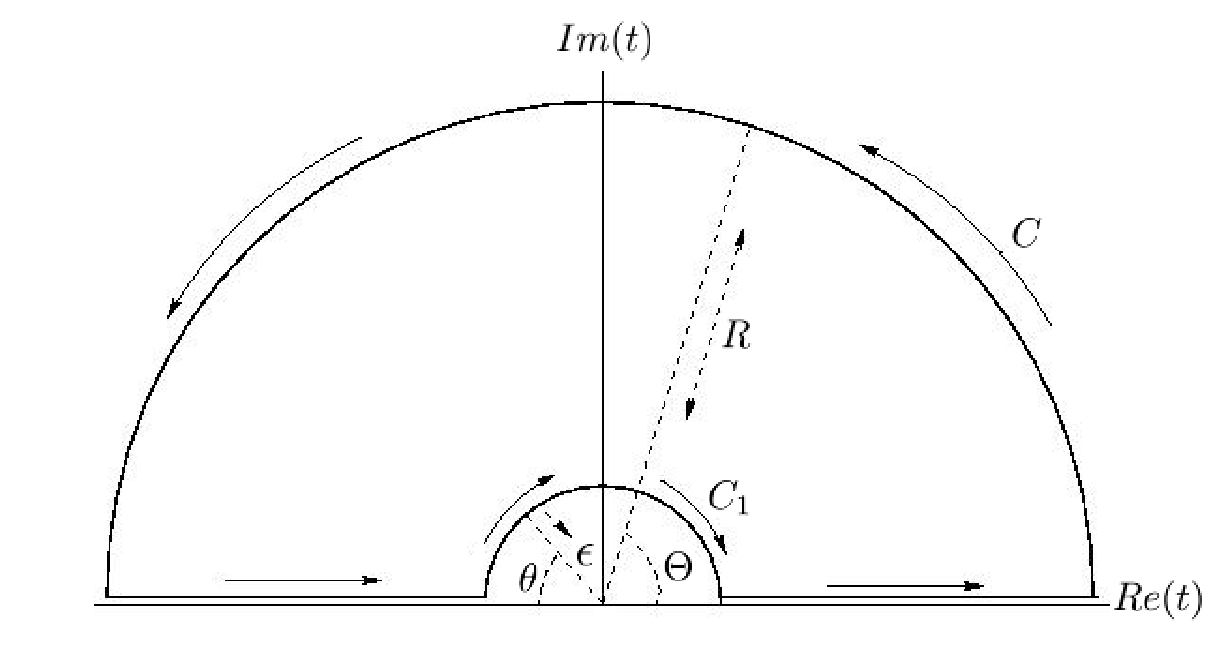
\psfig{file=jpegs/chapter-intro/fig_contours.eps,height=3.0in,width=5.0in}
\caption{Contours chosen for the integrals in Eqns~\ref{eq:int1:chapter-intro} and~\ref{eq:eqn4lnB:chapter-intro} in the complex plane. The radius $R \rightarrow \infty$ is the radius of the contour $C$, and the radius $\epsilon \rightarrow 0$ is the radius of the contour $C_1$. The angles of a particular point on $C$ and $C_1$ are denoted by $\Theta$ and $\theta$ respectively.}
\label{fig:contours:chapter-intro}
\end{figure}

\section{Three Level STIRAP}
\label{chapter-intro:section:stirap}
Stimulated Raman Adiabatic Passage, or STIRAP,  is a well-known method of inducing coherent excitations of quantum systems from the ground state to states with higher energy. This is achieved using coherent time-modulated laser fields that result in complete population transfer from an initially populated ground state to a target state via an intermediate state (see Fig~\ref{fig:3lvl:stirap:chapter-intro}). STIRAP was first proposed by Hioe and coworkers~\cite{stirap:hioe}~\cite{hioe:rwa:stirap}.  A crucial preliminary work by Becker, Gaubatz, Jones and Bergmann that achieved efficient vibrational excitation by using the molecular beam as an optically pumped active medium in a laser, led to the development of the STIRAP concept~\cite{stirap:seminal}. The theoretical work was formulated by Kuklinsky, Gaubatz, Hioe and Bergmann shortly thereafter~\cite{stirap:theory}. STIRAP was further confirmed by manipulating the vibrational and rotational degrees of freedom in sodium dimers~\cite{stirap:experiment}. Since then, STIRAP has been used to understand a diverse range of matter-optics systems, ranging from molecular alignment~\cite{stirap:molecular}, and molecular rotation~\cite{na-reichl:mol-rot}, to the coherent acceleration of ultracold atom systems~\cite{holder:reichl:2res}. This dissertation analyzes chaos in the latter for interacting bosons. In this section, we will be looking at the dynamics of STIRAP for a simple three level system. In further chapters, we will be investigating the effects of deterministic chaos in this dynamics by analyzing the STIRAP dynamics of the full multilevel system. 
\begin{figure}
\ 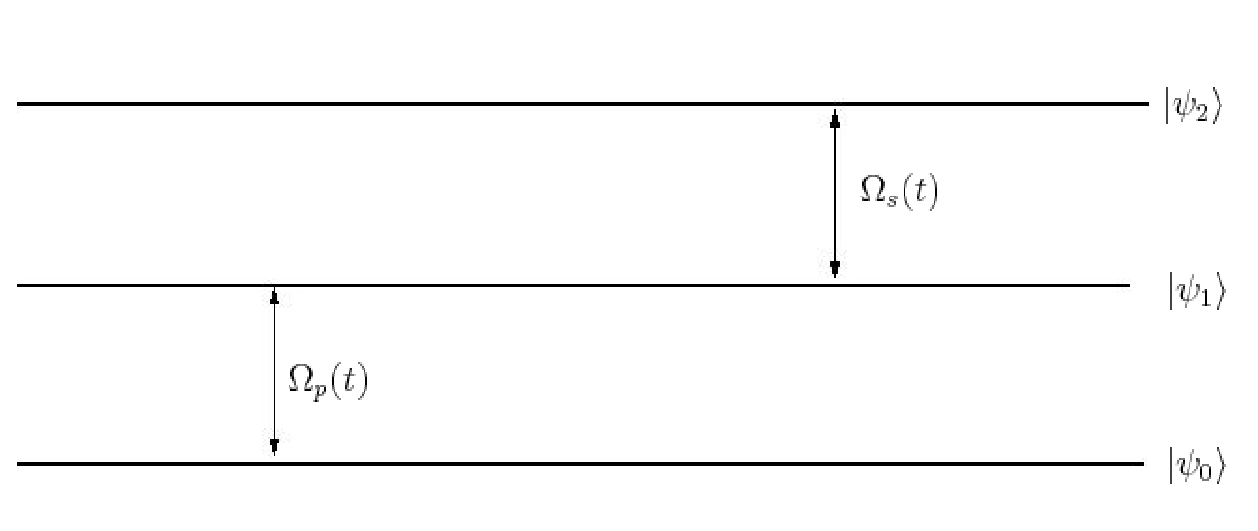
\psfig{file=jpegs/chapter-intro/fig_stirap.eps,height=3.0in,width=5.0in}
\caption{Linkage diagram for a three level Stimulated Raman Adiabatic Passage (STIRAP). A pump field of Rabi frequency $\Omega_p(t)$ and a Stoke field of Rabi frequency $\Omega_s(t)$ couple the states $\left \vert \psi_0\rangle , \vert \psi_1\rangle \right]$ and $\left[ \vert \psi_1\rangle, \vert \psi_2\rangle \right]$ respectively (as indicated by double arrows). If the Stoke field is switched on before the pump field, then the system, initially populated at $\vert \psi_0\rangle$, will achieve a complete population transfer to $\vert \psi_2\rangle$. The detunings $\Delta_{p,s}$ have been set to $0$.}
\label{fig:3lvl:stirap:chapter-intro}
\end{figure}
\subsection{Adiabatic time evolution}
For this simple three-level system, we denote the initial populated state at $t=-\infty$ by $|\psi_0\rangle$, the target state by $|\psi_2\rangle$, and the intermediate state by $|\psi_1\rangle$. The states  $|\psi_0\rangle$ and  $|\psi_1\rangle$ will be connected by a 'pump pulse' (of detuning $\Delta_p=0$), and the states  $|\psi_1\rangle$ and  $|\psi_2\rangle$ by a 'Stoke pulse' (of detuning $\Delta_s=0$). Figure~\ref{fig:3lvl:stirap:chapter-intro} illustrates the process with a linkage diagram for no detuning.
These pulses will have amplitudes that vary slowly in time from zero, to a peak value, then back to zero ('switching on' and then 'switching off'). Unlike other methods of excitations like optical pumping, this will be a two-photon resonance, similar to stimulated emission pumping, and the Stoke pulse will be switched on before the pump pulse.~\cite{stirap:hioe}~\cite{stirap:theory}~\cite{stirap:review}. Applying the R.W.A to this three-level system simplifies the Hamiltonian~\cite{hioe:rwa:stirap} to
\begin{equation}
H(t)=\hbar \left(
\begin{array}{ccc}
0 & \frac{1}{2}\Omega_p(t) & 0 \\
 \frac{1}{2}\Omega_p(t) & \Delta  & \frac{1}{2}\Omega_s(t)\\
 0 &  \frac{1}{2}\Omega_s(t) & 0
\end{array}
\right),
\label{eq:3lvl:stirap:hamilt:chapter-intro}
\end{equation}
where  $\Omega_{p,s}$  are the Rabi frequencies for the pump and Stoke pulses respectively, and describe the temporal profile of the switches (see Eqn~\ref{eq:rabifreq:chapter-intro}). Also, $\Delta=\Delta_p=\Delta_s$ is the single photon detuning of both pulses (necessarily kept equal). 

In the $\left[ |\psi_0\rangle, |\psi_1\rangle, |\psi_2\rangle  \right]$ basis, the adiabatic eigenvalues and eigenstates can be obtained by simply diagonalizing this Hamiltonian. The adiabatic eigenvalues of this Hamiltonian are
\begin{eqnarray}
\epsilon_0(t)=0, \nonumber \\
\epsilon_{\pm}(t) = \frac{1}{2}\left[ \Delta \pm \sqrt{\Delta^2 + \Omega'^2(t)}\right]. 
\label{eq:3lvl:evals:chapter-intro}
\end{eqnarray}
Solving the equations $H |\Phi_{0,\pm}\rangle = \epsilon_{0,\pm} |\Phi_{0,\pm}\rangle$ gives us
\begin{eqnarray}
|\Phi_+(t)\rangle = |\psi_0\rangle \sin{\theta(t)}\sin{\phi(t)} + |\psi_1\rangle \cos{\phi(t)}+|\psi_2\rangle \cos{\theta(t)}\sin{\phi(t)}, \nonumber \\
|\Phi_0(t)\rangle=|\psi_0\rangle \cos{\theta(t)} -|\psi_2\rangle \sin{\theta(t)}, \nonumber \\
|\Phi_-(t)\rangle = |\psi_0\rangle \sin{\theta(t)}\cos{\phi(t)} + |\psi_1\rangle \sin{\phi(t)}+|\psi_2\rangle \cos{\theta(t)}\cos{\phi(t)}.
\label{eq:3lvl:stirap:estates:chapter-intro}
\end{eqnarray}
Here, the mixing angles $\theta(t)$ and $\phi(t)$ are defined as
\begin{eqnarray}
\theta(t) \equiv \arctan{\frac{\Omega_p(t)}{\Omega_s(t)}}, \nonumber \\
\phi(t) \equiv \frac{1}{2} \arctan{\frac{\Omega'(t)}{\Delta}},
\label{eq:3lvl:mixang:chapter-intro}
\end{eqnarray}
and 
\begin{equation}
\Omega'(t)\equiv \sqrt{\Omega^2_p(t) + \Omega^2_s(t)}.
\label{eq:3lvl:omegap:chapter-intro}
\end{equation}
The state $|\Phi_0(t)\rangle$ has components only in the $\left[ |\psi_0\rangle , |\psi_2\rangle \right]$ subspace and no component in $|\psi_1\rangle$ and so is a trapped 'dark' state~\cite{stirap:review}. Thus, if we arrange it so that $\sin{\theta(t)}$ vanishes as $t \rightarrow -\infty$, and $\cos{\theta(t)}$ vanishes as $t \rightarrow \infty$, then $|\Phi_0\rangle$ will go from fully populating $|\psi_0\rangle$ to $|\psi_2\rangle$ as time evolves. From Eqns~\ref{eq:3lvl:mixang:chapter-intro}, we see that this is only possible if the mixing angle $\theta$ rises from $0$ to $\pi/2$ as time passes, meaning that the Rabi frequency and hence the amplitude (see Eqn~\ref{eq:rabifreq:chapter-intro}) of the Stoke pulse, $\Omega_s(t)$ must exceed that of the pump pulse, $\Omega_p(t)$ at earlier times. Therefore, the pulses must be applied in the counterintuitive 'Stoke first' order as described above for a complete population transfer to take place.

Figure~\ref{fig:evol:chapter-intro}.a through Fig~\ref{fig:evol:chapter-intro}.c shows plots for the system as it evolves through the STIRAP process in time $t$ (expressed in units of $t_{tot}$) with  $\Delta=0$. Figure~\ref{fig:evol:chapter-intro}.a shows plots for the Rabi frequencies $\Omega_p(t)$ and $\Omega_s(t)$, where the time dependence is chosen to be Gaussian ie $\Omega_{p,s}(t)=\Omega_0 e^{-(t-t_{p,s})^2/(2t^2_d)}$, with $t_s<t_p$. Thus, the Stoke pulse is 'switched on' before the pump pulse in the counterintuitive order. Figure~\ref{fig:evol:chapter-intro}.b shows the time evolution of the adiabatic eigenstates $\epsilon_{0,\pm}$ from Eqn~\ref{eq:3lvl:evals:chapter-intro}. Note the three-level avoided crossing at $t=0.5$ $t_{tot}$ where the dark state $|\Phi_0\rangle$ exchanges character with a linear combination of the $|\Phi_{\pm}\rangle$ states to finally obtain the character of $|\psi_2\rangle$. This is verified by Fig~\ref{fig:evol:chapter-intro}.c. In this figure, the evolution of the dark state $|\Phi_0\rangle$ is plotted as a function of time. The probabilities $P_i = |\langle \psi_i |\Phi_0\rangle|^2$ are shown for states $|\psi_0\rangle$ and $|\psi_2\rangle$ (see Eqns~\ref{eq:3lvl:stirap:estates:chapter-intro}). The population transfer from $|\psi_0\rangle$ to $|\psi_2\rangle$ is clearly seen at $t=0.5$ $t_{tot}$.

\begin{figure}
\ \psfig{file=jpegs/chapter-intro/fig_evol.eps, height=5.2in, width=3.5in}
\caption{Time evolution of the three level STIRAP problem. Figure (a) shows the Rabi frequency plots for the pump pulse $\Omega_p$, and Stoke  pulse $\Omega_s$ (scaled 
w.r.t $\Omega_0$) as functions of time $t$. The pulses have a Gaussian time dependence, with $t_s=(1/3)$, and $t_p=(2/3)$. The pulse widths of both pulses are $t_d=(1/10)$. Figure (b) shows the time dependence on the adiabatic eigenvalues $\epsilon_{0,\pm}$ of the Hamiltonian in Eqn~\ref{eq:3lvl:stirap:hamilt:chapter-intro} (see Eqn~\ref{eq:3lvl:evals:chapter-intro}). Figure (c) shows the time evolution of the dark state $|\Phi_0\rangle$ in Eqn~\ref{eq:3lvl:stirap:estates:chapter-intro} by plotting the occupation probability $P_i$ in undriven state $|i\rangle$. At $t=0$, it starts from a fully populated ground state $|0\rangle$ and switches character midway to fully populate $|2\rangle$, thereby achieving STIRAP. In all cases, the time is expressed in arbitrary units of $t_{tot}$. the detuning $\Delta=0$}
\label{fig:evol:chapter-intro}
\end{figure}

\subsection{Adiabaticity criterion}

We note that this evolution will be followed by the system in the strictly adiabatic limit, when no diabatic transitions take place between the eigenstates on account of time dependence. Thus, the system will be temporally adiabatic enough to follow this profile if the eigenstates of Eqns~\ref{eq:3lvl:stirap:estates:chapter-intro} are orthogonal compared to the eigenvalue differences~\cite{stirap:theory}~\cite{stirap:review} ie
\begin{equation}
|\langle \frac{d\Phi_0}{dt}|\Phi_\pm\rangle| \ll |\epsilon_0-\epsilon_\pm|.
\end{equation}
Simplifying the above for $\Delta=0$ gives us
\begin{equation}
\Omega'(t)\gg |\frac{d\theta(t)}{dt}|.
\label{eq:stirap:adiabaticity:chapter-intro}
\end{equation}
We assume that the Rabi frequencies vary in time as Gaussians, ie
\begin{equation}
\Omega_{p,s}(t) = \Omega_0 e^{-\beta (t-t_{p,s})^2} ,
\end{equation}
with $t_s>t_p$ so that the stoke pulse is 'switched on' first. Plugging the above equation into From Eqns~\ref{eq:3lvl:mixang:chapter-intro} and~\ref{eq:3lvl:omegap:chapter-intro} and applying Eqn~\ref{eq:stirap:adiabaticity:chapter-intro}, we get 
\begin{equation}
\Omega_0 \gg \left( 2\beta \right) \Gamma(t, t_s, t_p, \beta),
\label{eq:inequality:chapter-intro}
\end{equation}
where
\begin{equation}
\Gamma(t,t_s, t_p, \beta) \equiv \left( t_s - t_p \right) \frac{e^{-\beta (t-t_p)^2}e^{-\beta (t-t_s)^2}}{\left[ e^{-2\beta(t-t_s)^2} + e^{-2\beta(t-t_p)^2}     \right]^{3/2}}.
\end{equation}
Now, $t_s>t_p$ for a complete population transfer. If we use a time scale for the total time for both the pulses to traverse (denoted by $t_{tot}$), and scale all the time scales in $\Gamma$ , including the pulse widths $t_d \equiv 1/(\sqrt{2\beta})$,  by $t_{tot}$, then $(t_s-t_p)<t_{tot}$. If $t<t_s$, then we can simplify $\Gamma$ to the expression below. Thus,
\begin{equation}
\Gamma(t,t_s,t_p,\beta) = \left( t_s-t_p \right) \frac{e^{-\beta (t-t_p)^2}e^{2 \beta (t-t_s)^2}}{\left[ 1 + \frac{e^{-2\beta(t-t_p)^2}}{e^{-2\beta(t-t_s)^2}}     \right]^{3/2}}<t_{tot} 
\end{equation}
if $t_d \ll t_{s,p}$. Similarly, we can interchange $t_p$ for $t_s$ in the above expression for the range $t_s<t<t_p$ and arrive at the same conclusion. A similar argument can be made for $t_p<t<t_{tot}$ as well. Thus, in general, $\Gamma<t_{tot}$ and so can be eliminated from the inequality in Eqn.~\ref{eq:inequality:chapter-intro} to get the simple result
\begin{equation}
\Omega_0 t_d \gg \frac{t_{tot}}{t_d}.
\end{equation}
Since $t_d \ll t_{tot}$, it follows that $\Omega_0 t_d \gg 1$ is sufficient for the condition above to hold. Since the area of a Gaussian pulse is of the order of $\Omega_0  (t_d/t_{tot})$, it follows that the area of the pulse should be much greater than unity for adiabaticity to hold true. This will be a significant point in later chapters where actual pulse amplitudes need to be adjusted for the double well system.
